\begin{figure}
\centering
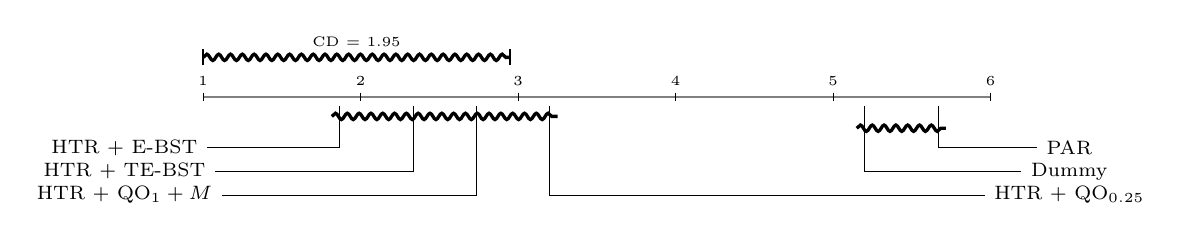
\begin{tikzpicture}[xscale=2]
\node (Label) at (1.973460322766162, 0.7){\tiny{CD = 1.95}}; % the label
\draw[decorate,decoration={snake,amplitude=.4mm,segment length=1.5mm,post length=0mm},very thick, color = black] (1.0,0.5) -- (2.946920645532324,0.5);
\foreach \x in {1.0, 2.946920645532324} \draw[thick,color = black] (\x, 0.4) -- (\x, 0.6);
 
\draw[gray, thick](1.0,0) -- (6.0,0);
\foreach \x in {1.0,2.0,3.0,4.0,5.0,6.0} \draw (\x cm,1.5pt) -- (\x cm, -1.5pt);
\node (Label) at (1.0,0.2){\tiny{1}};
\node (Label) at (2.0,0.2){\tiny{2}};
\node (Label) at (3.0,0.2){\tiny{3}};
\node (Label) at (4.0,0.2){\tiny{4}};
\node (Label) at (5.0,0.2){\tiny{5}};
\node (Label) at (6.0,0.2){\tiny{6}};
\draw[decorate,decoration={snake,amplitude=.4mm,segment length=1.5mm,post length=0mm},very thick, color = black](1.8166666666666664,-0.25) -- (3.2500000000000004,-0.25);
\draw[decorate,decoration={snake,amplitude=.4mm,segment length=1.5mm,post length=0mm},very thick, color = black](5.15,-0.4) -- (5.716666666666667,-0.4);
\node (Point) at (1.8666666666666665, 0){};\node (Label) at (0.5,-0.65){\scriptsize{HTR + E-BST}}; \draw (Point) |- (Label);
\node (Point) at (2.3333333333333335, 0){};\node (Label) at (0.5,-0.95){\scriptsize{HTR + TE-BST}}; \draw (Point) |- (Label);
\node (Point) at (2.733333333333333, 0){};\node (Label) at (0.5,-1.25){\scriptsize{HTR + QO$_{1} + M$}}; \draw (Point) |- (Label);
\node (Point) at (5.666666666666667, 0){};\node (Label) at (6.5,-0.65){\scriptsize{PAR}}; \draw (Point) |- (Label);
\node (Point) at (5.2, 0){};\node (Label) at (6.5,-0.95){\scriptsize{Dummy}}; \draw (Point) |- (Label);
\node (Point) at (3.2000000000000006, 0){};\node (Label) at (6.5,-1.25){\scriptsize{HTR + QO$_{0.25}$}}; \draw (Point) |- (Label);
\end{tikzpicture}
\caption{Nemenyi - main RMSE.csv}
\label{fig:nemenyi}
\end{figure}
